\documentclass[a4paper]{article}

\usepackage[english]{babel}
\usepackage[utf8]{inputenc}
\usepackage{amsmath}
\usepackage{graphicx}
\usepackage[colorinlistoftodos]{todonotes}
\usepackage{listings}
\addtolength{\textwidth}{1in}
\addtolength{\oddsidemargin}{-.5in}

\title{System Validation 2016 \\ Homework Part 1 - JML}

\author{Koen Mulder (s1757679) and Ruben van den Berg (s1354914)}

\date{\today}

\begin{document}
	\maketitle
	
	\begin{abstract}
		This homework assignment is done for the course System Validation. Here has been practiced with JML Annotations, Runtime Assertion Checking(from now on called RAC), Static Checking and Test Generation. In the first part JML annotations were made for informal array requirements. In the second part a game of Sokoban was used where informal requirements were made formal and were checked by JML Annotations, RAC, Static Checking and Test Generation. In the end the program behaved accordingly to the informal requirements. 
	\end{abstract}
	
	\section{Array Requirements}
	The first exercise relates to the array specification exercise as given in the first exercise session of the course. Below all informal requirements are given and a JML specification to solve this.
	\begin{itemize}
		\item Consider an array $B$ with $n$ elements: $B[0], . . . , B[n-1]$.
		All elements in $B$ are integers. Let $j$, $k$ be two indices such that $0 \leq j < k < n$.
		With $B[j], . . . , B[k]$ we denote the segment of $B$ starting from index $j$ and ending with index $k$. Which is in JML specifications
		\begin{lstlisting}
/*@ spec_public */ private int[]B;	// The array
/*@ spec_public */ private int n;	// Lenght of the array
/*@ spec_public */ private int j;	// Index start
/*@ spec_public */ private int k;	// Index end
		
//@ public invariant j >= 0 && j < k && k < n;
		\end{lstlisting}
		
		\item Any value that occurs in the segment $B[j], . . . ,B[k]$ also occurs outside that segment.
		\begin{lstlisting}
//@ public invariant (\forall int i1; i1 >= j && i1 <= k;
(\exists int i2; (i2 >= 0 && i2 < j) || (i2 > k && i2 < n); B[i1] == B[i2]));
		\end{lstlisting}
		This is checked by going over this segment and see if there is a match for every element outside of $B[j], . . . , B[k]$
		
		\item The array $B$ does not contain duplicates when the segment $B[j], . . . , B[k]$ is not considered.
		\begin{lstlisting}
//@ public invariant (\forall int i1, i2; i1 >= 0 && i2 > i1 && i2 < n;
(B[i1] == B[i2]) ==> ((i1 >= j && i1 <= k) || (i2 >= j && i2 <= k)));
		\end{lstlisting}
		If there are two elements who are duplicates of each other it must mean one of the elements is inbetween $B[j], . . . , B[k]$.
		
		\item Any value occurs at most twice in B.
		\begin{lstlisting}
//@ public invariant (\forall int i1,i2,i3; i1>=0 && i2>i1 && i3>i2 && i3<n;
B[i1] != B[i2] || B[i2] != B[i3] || B[i1] != B[i3]);	
		\end{lstlisting}
		If you have three values at least two values can not be equal to eachother.
		
		\item The highest value occuring in B occurs at least twice in B.
		\begin{lstlisting}
//@ public invariant (\exists int i1, i2; i1 >= 0 && i2 > i1 && i2 < n;
B[i1] == B[i2] && (\forall int i3; i3 >= 0 && i3 < n; B[i1] >= B[i3]));	
		\end{lstlisting}
		First we check if two elements are the same. If so we check for all other elements if they are equal or higher then those elements.
		
		\item The array B contains a palindrome of length k.
		\begin{lstlisting}
//@ public invariant (\exists int i1, i2; i1 >= 0 && i2 == (i1+k-1) && i2 < n;
(\forall int i3; i3 >= 0 && i3 < k; B[i1 + i3] == B[i2 - i3]));	
		\end{lstlisting}
		Index i1 and i2 are a segement with lenght k, after this we check for the palindrome. We consider the segment i1,i2 a sub array. We use two indices to check from back to front and the other way around. For every possible itteration the elements for these indices should be the same.
		
		\item After doing at most one swap the array B is sorted.
		\begin{lstlisting}
/*@ public invariant (\exists int i1, i2; i1 >= 0 && i2 > i1 && i2 < n;
(\forall int i3; i3 >= 1 && i3 < n; 
B[i3-1] <= B[i3] || (i3 == i1 && B[i3-1] <= B[i2]) ||
(i3-1 == i2 && B[i1] <= B[i3]) || (i3-1 == i1 && i3 == i2 && B[i2] <= B[i1])));
@*/
		\end{lstlisting}
		We take two different indices(i1 and i2). Next we check every element in the array against the element in front. For every pair we check if the second element value is bigger or equal to the first. If this is not the case we check if the array will be sorted when i1 and i2 are swapped. 
		
		\item There is a value that occurs more often in B than any other value.
		\begin{lstlisting}
/*@ public invariant (\exists int i1; i1 >= 0 && i1 < n;
(\forall int i2; i2 >= 0 && i2 < n && B[i1] != B[i2]; 
(\sum int s1; s1 >= 0 && s1 < n && B[s1] == B[i1]; 1) >
(\sum int s2; s2 >= 0 && s2 < n && B[s2] == B[i2]; 1) ) );
@*/
		\end{lstlisting}
		We take an index and check for every other index which does not have the same element value. If the first element value always occurs more often the statement holds.
		
	\end{itemize}
	\newpage
	
	\section{JML Annotations and Runtime Assertion Checking}
	The goal in this part of the assignment was to turn informal requirements into JML specifications, these were marked with \texttt{@informal} in the inline comments in the code. For doing this we mainly used \texttt{invariant, requires, ensures} and \texttt{assignable} were mostly used to create the JML specifications. Only in the \texttt{boolean movePlayer (Position newPosition)} method \texttt{assert} is used to create assertion in methods itself. This part is split up into 2 parts, the JML annotations and the runtime assertion checkers. In the first part the most important annotations are shown per class, less interesting or basic annotations are only briefly mentioned. In the runtime assertion checking part the results of runing the program with these annotation is discussed.

	\subsection{JML Annotations}
	\label{subsec:jmlspec}
	\subsubsection{Position}
	The first assertions added are in the \texttt{class Position}, these are used mainly for checking if a positions is valid. This firstly includes invariants that state that x and y are always 0 or more. Similar assertions are used for checking the input in the constructor.
	\begin{lstlisting}
//@ invariant x >= 0 && y >= 0;
	\end{lstlisting}
	The other applications of assertions in the \texttt{class Position} is for the method \texttt{boolean isValidNextPosition (Position newPosition)}. 
	\begin{lstlisting}
//@ requires Math.abs(newPosition.x - x) + Math.abs(newPosition.y - y) == 1;
//@ ensures \result == true;
//@ also
//@ requires Math.abs(newPosition.x - x) + Math.abs(newPosition.y - y) != 1;
//@ ensures \result == false;
	\end{lstlisting}
	Assertions are also added to the equals method and to the constructor, in which they state that the $x$ and $y$ values are set to the parameters.
	
	\subsubsection{Player}
	Assertions added the \texttt{class Player} are all basic. To the constructor assertions are added to state that the position parameter is the same as the position of the player. To \texttt{public void setPosition (Position newPosition)} annotations are added that state the new position is valid and that position of the player equals the parameter.
	\begin{lstlisting}
//@ requires position.isValidNextPosition (newPosition);
//@ ensures this.position.equals (position);
	\end{lstlisting} 
	
	\subsubsection{BoardItem}
	In \texttt{class BoardItem} invariants are added to state that if an item is a crate or is marked, it has to be ground. These specifications originate from the \texttt{class Board}.
	\begin{lstlisting}
	//@ public invariant crate ==> ground;
	//@ public invariant marked ==> ground;
	\end{lstlisting}
	
	\subsubsection{Board}
	To the class \texttt{class Board} several assertions are added in ration to the size and state of the board.
	\begin{lstlisting}
//@ public invariant xSize > 0 && ySize > 0;
//@ public invariant xSize == ySize;
//@ public invariant xSize == items.length;
//@ public invariant \forall int x; x >= 0 && x < items.length; 
		ySize == items[x].length;
//@ public invariant \nonnullelements (items);
//@ public invariant \forall int x; x >= 0 && x < items.length; 
		\nonnullelements(items[x]);
	\end{lstlisting}
	It is stated that the xSize and ySize need to be equal and both greater then zero, the dimensions of the array need to match the xSize and ySize and finally the elements in the array are not allowed to be \texttt{null}. The last 3 of these annotations are added because of problems that occurred during the Static checking (\ref{sec:staticchecking}).
	Annotations are added to the constructor to ensure the dimensions are valid and the array is filled with walls.
	\begin{lstlisting}
//@ assignable items;
//@ assignable this.xSize;
//@ assignable this.ySize;
//@ requires xSize > 0 && ySize > 0 && xSize == ySize;
//@ ensures \forall int x; x >= 0 && x < xSize; \forall int y; y >= 0 && y < ySize; 
		items[x][y].ground == false;
//@ ensures items.length == xSize && items[0].length == ySize;
	\end{lstlisting}
	Annotations added to \texttt{public boolean onBoard(Position p)}:
	\begin{lstlisting}
//@ ensures \result == (0 <= p.x && p.x < xSize && 0 <= p.y && p.y < ySize);
	\end{lstlisting}
	And annotations added to the \texttt{public boolean isOpen(Position p)}:
	\begin{lstlisting}
//@ requires onBoard(p);
//@ ensures \result == (items[p.x][p.y].ground && !items[p.x][p.y].crate);
//@ also
//@ requires !onBoard(p);
//@ ensures \result == false;
	\end{lstlisting}
	The annotations for both the \texttt{(Position p)} variant or the \texttt{(int x, int y)} variant are almost the same, with the only difference to the input variable against which is checked.
	
	\subsubsection{Game}
	The most important annotations int \texttt{class Game} are related to the \texttt{boolean wonGame ()} and \texttt{movePlayer (Position newPosition)}. The annotations added to \texttt{boolean wonGame ()} check if the result is true if all marked positions also are a crate. The annotation used in this methods are further explained in \ref{sec:staticchecking} Static Checking.
	\begin{lstlisting}
//@ ensures \result == (\forall int x; x >= 0 && x < board.xSize; 
	(\forall int y; y >= 0 && y < board.ySize;
		board.items[x][y].marked ==> board.items[x][y].crate));
	\end{lstlisting}
	The annotations to \texttt{movePlayer (Position newPosition)} are the most extensive annotations of the project, other then pre and post conditions multiple assertions are added to the body of the method.
	\begin{lstlisting}
//@ normal_behaviour
//@ requires !player.position.isValidNextPosition (newPosition);
//@ ensures \result == false;
//@ also normal_behaviour
//@ requires !board.onBoard(newPosition);
//@ ensures \result == false;
//@ also normal_behaviour
//@ requires !board.items[newPosition.x][newPosition.y].ground;
//@ ensures \result == false;
//@ also normal_behaviour
//@ requires board.isOpen(newPosition);
//@ requires player.position.isValidNextPosition (newPosition);
//@ requires board.onBoard(newPosition);
//@ ensures \result == true;
//@ also normal_behaviour
//@ requires board.onBoard(newPosition);
//@ requires board.items[newPosition.x][newPosition.y].crate;
//@ requires player.position.isValidNextPosition (newPosition);
//@ requires board.isOpen(newPosition.x + (newPosition.x - player.position.x), 
	newPosition.y + (newPosition.y - player.position.y));
//@ ensures \result == true;
//@ also normal_behaviour
//@ requires board.onBoard(newPosition);
//@ requires board.items[newPosition.x][newPosition.y].crate;
//@ requires player.position.isValidNextPosition (newPosition);
//@ requires !board.isOpen(newPosition.x + (newPosition.x - player.position.x), 
	newPosition.y + (newPosition.y - player.position.y));
//@ ensures \result == false;
	\end{lstlisting}
	The annotations check for all the different situations that can happen within the method such as invalid positions, walls, boxes and they can be pushed or not.
	
	\subsection{Runtime Assertion Checking}
	The following problems were found during runtime checking:
	\begin{itemize}
		\item Players could move through walls.
		\item Diagonal movement was a valid next position.
		\item The current position is a valid next position.
	\end{itemize}
	The first problem found was that players had the ability to move through walls. This problem was detected both visually and by the JML checker. The problem occurs in the \texttt{class Game} inside the method \texttt{boolean movePlayer (Position newPosition)}. This class method has a list of mutiple JML specifications for 6 different situations. The following specification detected the problem:
	\begin{lstlisting}
//@ requires !board.items[newPosition.x][newPosition.y].ground;
//@ ensures \result == false;
	\end{lstlisting}
	This states that a move to a position that is not ground is not a valid move and will not be executed. At runtime it was found that this was not the case and that a player was able to move to a position that is not ground. After adding an check in \texttt{boolean movePlayer (Position newPosition)} which validates that the \texttt{newPosition} should be on a ground position the code functions according to the specification.
	
	The next problem was ability of the player to move diagonally to another position. This is in contract with the specification which states: \textbf{\textit{a valid next position is always one move horizontally or vertically from the current one}}. As the previous problem this was also detected visually and by the JML checker. This problem was detected in the \texttt{class Position} in the method \texttt{boolean isValidNextPosition (Position newPosition)}. Part of the JML specification is as follows:
	\begin{lstlisting}
//@ requires Math.abs(newPosition.x - x) + 
Math.abs(newPosition.y - y) == 1;
//@ ensures \result == true;
	\end{lstlisting}
	There also is an additional part in which the requires expression is not equal to 1, in that case it should return false. By changing the way the method checks if a position is valid of not this problem was was repaired.
	
	The final problem was discovered based on the same specification as the second problem. According the code the current position of the player was also a valid next position, but according to the specification this is not the case. This problem was solved when the second problem was solved.
	
	\newpage
	\section{Static Checking}
	\label{sec:staticchecking}
	Within this section we will perform formal verification on the method \texttt{wonGame} in the \texttt{Game} class. The \texttt{wonGame} method is responsible for checking the winning situation on the game board after every move.
	\newline 
	We implemented four \texttt{loop invariants}, two per for loop. One describing if the $x$ or $y$ element was within the correct boundaries, the other is a nested \texttt{forall} loop checking the result. The loop invariant for the outer loop iterating of the $x$ was as following:
	\begin{lstlisting}
//@ loop_invariant x >= 0 && x <= board.xSize;
//@ loop_invariant result == \forall int i; i >= 0 && i < x; 
	(\forall int j; j >= 0 && j < board.ySize; 
		!board.items[i][j].marked || board.items[i][j].crate);
//@ decreases board.xSize - x;
	\end{lstlisting}
	The loop invariant for the inner loop iterating of the $y$ was as following:
	\begin{lstlisting}
//@ loop_invariant y >= 0 && y <= board.ySize;
//@ loop_invariant rowresult == (\forall int i; i >= 0 && i < y; 
	!board.items[x][i].marked || board.items[x][i].crate);
//@ decreases board.ySize - y;
	\end{lstlisting}
	
	A problem we encountered during the implementation of the nested \texttt{forall} loop was the nonzero error. Within the loop elements could not be zero. We fixed this by adding the following specifications to Board.java.
	\begin{lstlisting}
//@ public invariant \forall int x; x >= 0 && x <
    items.length; ySize == items[x].length;
//@ public invariant \nonnullelements (items);
//@ public invariant \forall int x; x >= 0 && x <
    items.length; \nonnullelements(items[x]);	
	\end{lstlisting}
	Here we state that every item can not be \texttt{null}. Same goes for all the items in the sub-array. Next we state that the \texttt{ySize} needs to be equal to \texttt{items[x].length} when $x$ is between zero and \texttt{items.length}. 
	\newline
	We did not encounter any more errors afterwards in the \texttt{WonGame} method. However still some errors occured in the \texttt{MovePlayer(Position)} method when static checked. This is acceptable since this method is fully checked during runtime without any errors. Due to the complexity of the method and the specification we are not sure how to solve these erros given by the static checker at the \texttt{MovePlayer(Position)} method.
	
	If we would get a similar assignment in which we had to specify loop invariants we would probably do it the same way. In the case of multiple loops we would works from inside out, starting with most inner loop, annotating it, moving on the the loop around it. In each of these iterations you would reason about what will make the check either true or false and turn this into loop invariants together with the limiting invariants and decreases.
	
	\section{Test Generation}
	The goal of this part of the exercise was generate tests for the JML specifications and provide test data to feed these generates tests.
	For this part of the exercise we did not create any additional JML annotations in the code as we did already create the required specification in \ref{subsec:jmlspec} \textit{JML Annotations and Runtime Assertion Checking: JML Annotations}.
	The first created a set of different \texttt{Game} objects with a \texttt{Board} and \texttt{Player}, each \texttt{Game} object was created for a different situation, those are summed below:
	\begin{itemize}
		\item moving to ground position
		\item moving to a marked ground position
		\item moving to a wall position
		\item moving towards a wall in different situations
		\begin{itemize}
			\item a wall with ground behind it
			\item a wall with marked ground behind it
			\item a wall with a wall behind it
			\item a wall with an other box behind it
		\end{itemize}
	\end{itemize}
	All the \texttt{Board}s had a size of 7 by 7 with the player starting in the center.
	
	The next step was to create position data to feed to the \texttt{movePlayer(Position newPosition)}. For this we just created all possible combination for $x$ and $y$ with the value 0 to 7(inclusive), resulting in 64 positions. This means that we provide more positions then the test boards contains. By using these positions we also run all kinds different scenarios such as diagonal movement, movement too far away and movement to invalid positions. No negative positions were used as this is in conflict with the specification of \texttt{Position}. We ended up with 196 successfully completed tests.
	
	\begin{figure}[h]
		\centering
		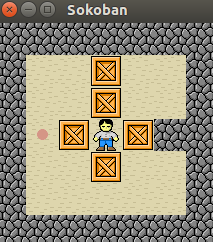
\includegraphics[]{Sokoban.png}
		\caption{A test board for Sokoban (crates)}
	\end{figure}

	\begin{figure}
		\centering
		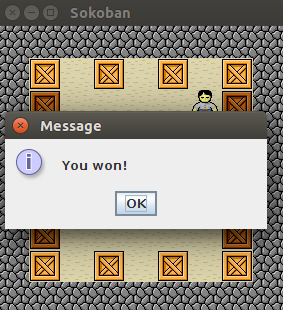
\includegraphics[]{Sokobanwin.png}
		\caption{Sokoban win}
	\end{figure}
	
\end{document}
